

%----------------------------------------------------------------%
\section[Prelinaries]{Preliminaries}
%---------------------------------------------------------%

\begin{frame}{\bf \tcb{Introduction to GGplot}}
Basic Commands

\begin{itemize}\itemsep0.3cm
\item Use a recent release of \texttt{R}. Managing package is more or less same as other packages.
\item Based on the ``Grammar of Graphics"
\item \texttt{qplot()} Quickplot
\item \texttt{ggplot()}

\end{itemize}
\end{frame}
\begin{frame}{\bf \tcb{Types of Plots}}

\begin{itemize}\itemsep0.3cm
\item Bar Plots and Bar Charts / Pie Charts
\item Time Series Line Plots
\item Scatterplots
\item Histograms
\item Density Plots
\end{itemize}
\end{frame}
%----------------------------------------------------------------%

%----------------------------------------------------------------%
\begin{frame}{\bf \tcb{Overview of Wickham's Book}}
\begin{itemize}\itemsep0.25cm
\item[1] Introduction
\item[2]
\item[3] The \textbf{\texttt{qplot()}} function
\item[4]
\item[5] Random Stuff
\item[6]
\item[7] Faceting
\item[8]
\end{itemize}
\end{frame}
%----------------------------------------------------------------%
\begin{frame}[fragile]{\bf \tcb{Fisher's Iris Data set}}
Fisher's Iris Data Set. Very simple Scatter plot
\begin{verbatim}

>
>qplot(Sepal.Length, Petal.Length, data = iris,
+ color = Species)
>
\end{verbatim}
\end{frame}

%----------------------------------------------------------------%
\begin{frame}{\bf \tcb{Scatterplot of Iris Data set}}
\vspace{-1cm}
\begin{center}
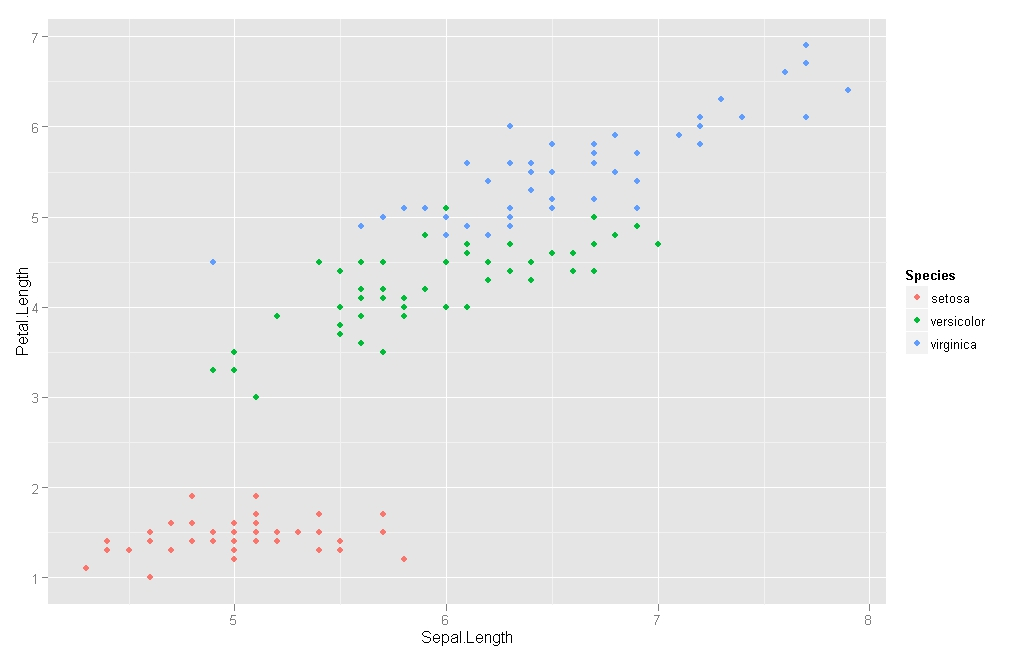
\includegraphics[scale = 0.35]{IrisPlot1}
\end{center}
\end{frame}
%---------------------------------------------------------%
\begin{frame}{\bf \tcb{What is a 'Geom'?}}
\begin{itemize}\itemsep0.37cm
\item What is a Geom? Geometric Object - such as a line or point.
\item The default is point. Lets use "line" (even though it doesn't make sense for this data).
\end{itemize}
\end{frame}
%----------------------------------------------------------------%
\begin{frame}[fragile]{\bf \tcb{Fisher's Iris Data set}}
enhancments
\begin{verbatim}
> qplot(Sepal.Length, Petal.Length, data = iris,
  geom="line", color = Species)
>
\end{verbatim}
\end{frame}
%----------------------------------------------------------------%
\begin{frame}{\bf \tcb{Scatterplot of Iris Data set}}
\vspace{-1cm}
\begin{center}
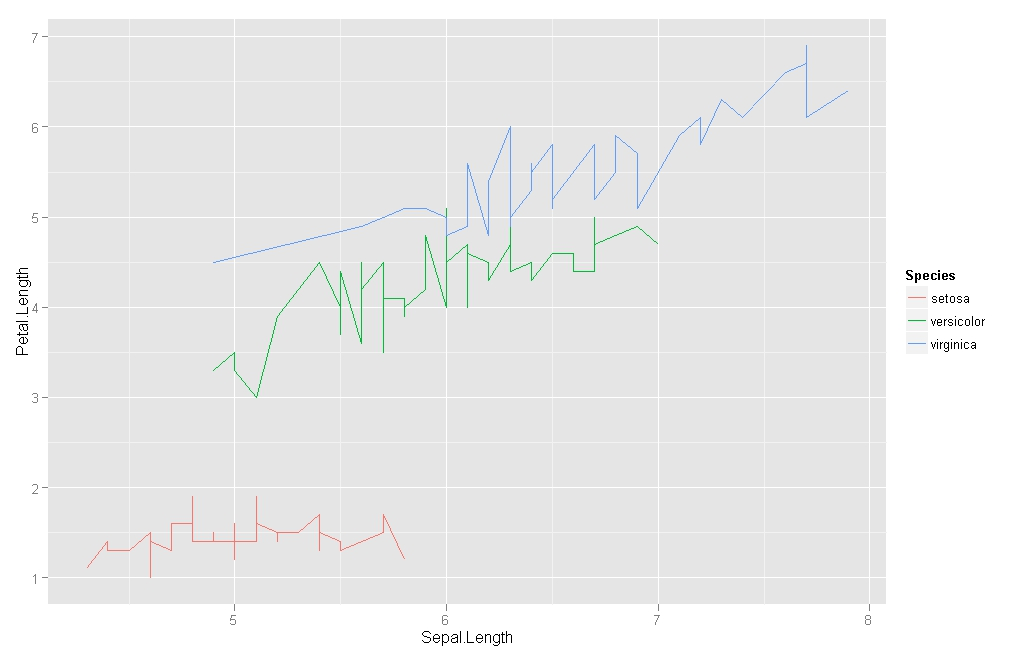
\includegraphics[scale = 0.35]{IrisPlot2}
\end{center}
\end{frame}

%----------------------------------------------------------------%
\begin{frame}[fragile]{\bf \tcb{MT Cars}}
\begin{itemize}
\item[disp] Displacement (kilograms)
\item[mpg] Miles Per Gallon 
\item[am] AM?? (Either 0 or 1)
\end{itemize}
\begin{verbatim}
>qplot(disp,mpg,data=mtcars,colour=am)
>
\end{verbatim}
\end{frame}


%----------------------------------------------------------------%
\begin{frame}{\bf \tcb{Scatterplot of MT Cars}}
\vspace{-1cm}
\begin{center}
\includegraphics[scale = 0.35]{cars2}
\end{center}
\end{frame}

%----------------------------------------------------------------%
\begin{frame}{\bf \tcb{Orange Trees}}
\vspace{-1cm}
\begin{center}
\includegraphics[scale = 0.35]{Orange1}
\end{center}
\end{frame}

%----------------------------------------------------------------%
\begin{frame}{\bf \tcb{Orange Trees}}
\vspace{-1cm}
\begin{center}
\includegraphics[scale = 0.35]{Orange2}
\end{center}
\end{frame}

%----------------------------------------------------------------%

\begin{frame}{\bf \tcb{Faceting}}
\begin{itemize}\itemsep0.7cm
\item What is `Facetting'?
\item Panel Data
\item Section 7 of Hadley Wickhams Book.

\end{itemize}
\end{frame}


\end{document}








%----------------------------------------------------------------%
\begin{frame}{\bf \tcb{Lesson Plan (continued)}}
\begin{itemize}\itemsep0.3cm
\item Repeat this experiment many times (or equivalently - everyone in the class performs the experiment independently). For the time being, consider only the summation.
\item Simple exercise: Table and histogram of (simulated) data, with discussion of the shape of the histogram (Bell-Shaped!)
\item For specialist students (Maths etc), examples of simple \texttt{R} code provided and explained.

\end{itemize}
\end{frame}


%----------------------------------------------------------------%
\begin{frame}[fragile]{\bf \tcb{Simple \texttt{R} Code}}
\begin{itemize}
\item Assuming very limited knowledge of programming.
\end{itemize}
\begin{verbatim}
> Dice <- 1:6       #Sample Space
> Dice
[1] 1 2 3 4 5 6
>
> X <- sample(Dice,100,replace=TRUE)
> sum(X)
[1] 342
>
> X <- sample(Dice,100,replace=TRUE)
> sum(X)
[1] 335
\end{verbatim}
\end{frame}
%----------------------------------------------------------------%
\begin{frame}{\bf \tcb{Frequency Tables (condensed)}}
\begin{itemize}
\item Suppose we repeat this experiment a large number of times (e.g. 2000 times).
\end{itemize}
\begin{center}
\begin{tabular}{|c|c|c|}
\hline
Class&Frequency&Rel. Fequency\\
  \hline
  % after \\: \hline or \cline{col1-col2} \cline{col3-col4} ...
  280-299 & 5 & 0.25$\%$ \\
  300-319 & 76 & 3.8 $\%$ \\
  320-339 & 465 & 23.25 $\%$ \\
  340-359 & 951 & 47.55 $\%$\\
  360-379 & 516 & 25.80$\%$\\
  380-399 & 64 & 3.2$\%$\\
  400-419 & 4 & 0.2$\%$ \\

  \hline
\end{tabular}
\end{center}
\end{frame}

%----------------------------------------------------------------%
\begin{frame}{\bf \tcb{Commentary of Die Experiment}}
\begin{itemize}\itemsep0.3cm
\item Commentary on the shape of the histogram, and distribution of summations.
\item Extend this idea to distribution of sample means.
\item Introduction of the concept of the \textbf{\emph{Central Limit Theorem}}.
\item Recall the die is known to be fair in these experiments.
\item Discussion on the ``extreme" results: would a summation of less than 300 or more than 400 be expected before the experiment started?
\item Introduction of the concept of the \textbf{\emph{p-value}}.
\end{itemize}
\end{frame}
%----------------------------------------------------------------%
\begin{frame}{\bf \tcb{Adjusting the Sample Size}}
\begin{itemize}\itemsep0.3cm
\item Previously used a sample size of 100.
\item Try out different samples sizes (i.e. n=50,200 etc).
\item Previously considered \textbf{\emph{summations}}, but now consider \textbf{\emph{means}} for ease of comparison.
\item How does changing the sample size relate to the precision?

\item Introduce the concept of the standard error of a statistic (and relationship to standard deviation).
\item For normal distributions: the $\sqrt{n}$ relationship.
\end{itemize}
\end{frame}

%----------------------------------------------------------------%

\begin{frame}{\bf \tcb{Progression: Crooked Die}}
\begin{itemize}\itemsep0.3cm
\item Repeat the procedure for a die known to be `crooked'.
\item Expected value of summations/means different. Otherwise similar to before.
\item Consider a die roll experiment where die is either of the following
 \begin{itemize} \item Possibly a fair die \item or possibly a `crooked die' that favours high values.
\end{itemize}
\item The experiment yields a summation of 380.
\item Do you think the die is fair or crooked?
\end{itemize}
\end{frame}

